% !TEX program = xelatex
%Wzór dokumentu
%tu zmień marginesy i rozmiar czcionki
\documentclass[a4paper,12pt]{article}
\usepackage{inputenc}[utf8]
\usepackage[margin=2.8cm]{geometry}
\usepackage[polish]{babel}

%Lepiej tego nie zmieniaj, jak co to dodawaj pakiety
\usepackage{titlesec}
\usepackage{titling}
\usepackage{fancyhdr}
\usepackage{mdframed}
\usepackage{graphicx}
\usepackage{amsmath}
\usepackage{amsfonts}
\usepackage{multicol}
\usepackage{multirow}
\usepackage{listings}
\usepackage{caption}
\usepackage{float}
\usepackage{pdfpages}
\usepackage{tikz}
	\usetikzlibrary{arrows}
	\usetikzlibrary{patterns}
	\usetikzlibrary{decorations.pathmorphing}
\usepackage{pgf}
\usepackage[section]{placeins}



%inny wygląd
%\usepackage{tgbonum}


\usepackage{hyperref}
\hypersetup{
    colorlinks=true,
    linkcolor=blue,
    filecolor=magenta,      
    urlcolor=cyan,
}

\urlstyle{same}
%Zmienne, zmień je!
\graphicspath{ {./ilustracje/} }
\title{Wyznaczanie wartości przyspieszenia ziemskiego metodą spadku swobodnego}
\author{Grzegorz Koperwas}
\date{\today}

%lokalizacja polska (odkomentuj jak piszesz po polsku)

\usepackage{polski}
\usepackage[polish]{babel} 
\usepackage{indentfirst}
\usepackage{icomma} 

\brokenpenalty=1000
\clubpenalty=1000
\widowpenalty=1000    

%nie odkometowuj wszystkiego, użyj mózgu
%\renewcommand\thechapter{\arabic{chapter}.}
\renewcommand\thesection{\arabic{section}.}
\renewcommand\thesubsection{\arabic{section}.\arabic{subsection}.}
\renewcommand\thesubsubsection{\arabic{subsubsection}.}

%Makra

\newcommand{\obrazek}[2]{
\begin{figure}[h]
    \centering
    \includegraphics[scale=#1]{#2}
\end{figure}
}     

\newcommand{\stopnie}{\ensuremath{^{\circ}}}

\newcommand{\twierdzonko}[1]{
    \begin{center}
    \begin{mdframed}
    #1
    \end{mdframed}          
    \end{center}
} 

\newcommand{\dwanajeden}[2]{
\ensuremath \left( \begin{array}{c}
    #1\\
    #2
\end{array} \right)
}  

%Stopka i head (sekcja której nie powinno się zmieniać)
\pagestyle{fancy}
\fancyhead{}
\fancyfoot{}

%Zmieniaj od tego miejsca
\rfoot{\thepage}
\lfoot{}
\lhead{}
\rhead{Ostatnia edycja: \today}
\renewcommand{\headrulewidth}{1pt}
\renewcommand{\footrulewidth}{1pt}



\begin{document}
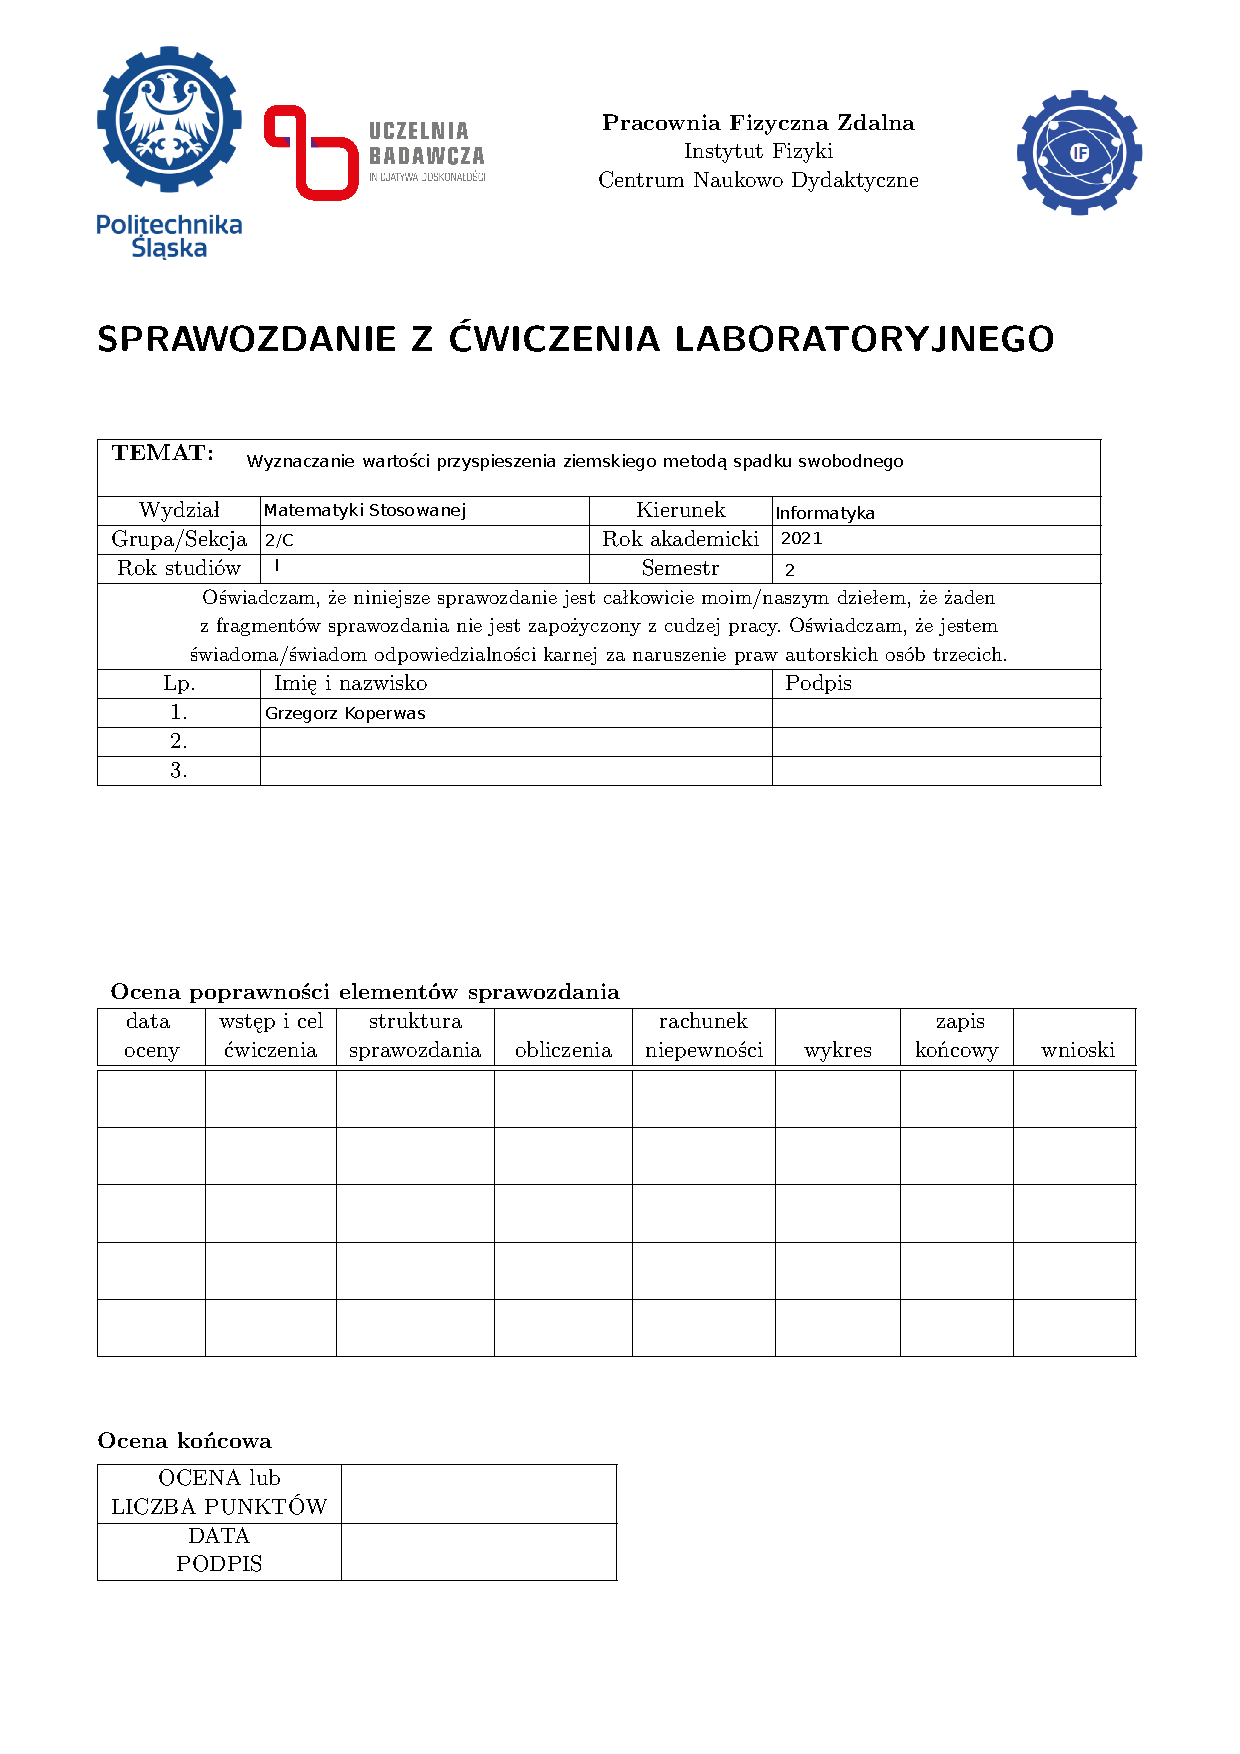
\includepdf[pages=-]{PFZ-StrTytulowa.pdf}

\section{Wstęp teoretyczny}

Celem doświadczenia jest pomiar przyspieszenia grawitacyjnego poprzez pomiar
czasu, jaki potrzebuje ciało do upadku z danej wysokości.

\begin{figure}[h]
	\begin{tikzpicture}
		\fill (-0.5, -0.5) rectangle (.5, .5);
		\draw [->] (0, -.5) -- (0, -2) node[right] {$\vec{F_g}$};
		\draw [pattern = north east lines, draw=none, fill] (-2, -4) rectangle (2, -4.2);
		\draw (-2, -4) -- (2, -4);
		\draw [<->, thin] (-.5, -.5) -- (-.5, -4) node[pos=.5, left] {$H$};
	\end{tikzpicture}
	\centering 
	\caption{Układ pomiarowy}
\end{figure}

Na ciało działa siła grawitacji $\vec{F_g}$, wprawiająca je w ruch z
przyspieszeniem $g$, zatem ruch tego ciała jest jednostajnie przyspieszony.
Mierzony jest czas $t$ w jakim ciało pokonuje odległość $H$. Ciało na początku
jest w spoczynku.

Równanie ruchu dla danego przypadku ma postać:

\[ H = \frac{gt^2}{2} \]

Zatem $g = \frac{2}{m}$ gdzie m to współczynnik nachylenia prostej o równaniu:

\begin{equation}
	t^2 = m \cdot H
\end{equation}

\clearpage
\section{Pomiary}

\subsection*{Metoda pomiarowa}

Pomiary były wykonywane inną metodą niż ta zalecona, zamiast aplikacji
\emph{PhysBox} wykorzystano program \emph{Audacity}, którym manualnie
analizowano nagrania z mikrofonu komputera. Czas upadku był wyznaczony jako
odstęp czasu między środkiem pierwszego dźwięku (suwania się ciała z poziomicy)
a dźwiękiem uderzenia ciała w podłogę.

Typowa długość pierwszego dźwięku została wyznaczona jako $0,08s$, zatem
niepewność czasu rozpoczęcia spadku swobodnego jest połową tej wartości. Jako iż
dźwięk upadku ciała o podłogę jest dużo głośniejszy i upadek występuje na jego
samym początku to jako nie pewność możemy użyć połowę okresu próbkowania
mikrofonu czyli około $1,1 \cdot 10^{-5}s$

Ostatecznie jako iż niepewność drugiego dźwięku jest znikoma w porównaniu do
niepewności pierwszego\footnote{Jeśli dodamy te niepewności to otrzymamy wartość
$0,040011s$, która po zaokrągleniu do dwóch cyfr znaczących daje nam $0,040s$},
to za niepewność pomiaru przyjmujemy $0,04s$.

\subsection*{Wyniki pomiarów:}

\begin{table}[h]
\centering
\begin{tabular}{|l|l|l|l|l|l|l|l|l|}
\hline
\multicolumn{1}{|c|}{\multirow{2}{*}{H [cm] $\pm 0,1cm$}} & \multicolumn{8}{c|}{t [s] $\pm 0,04s$}                \\ \cline{2-9} 
\multicolumn{1}{|c|}{} &
  \multicolumn{1}{c|}{1} &
  \multicolumn{1}{c|}{2} &
  \multicolumn{1}{c|}{3} &
  \multicolumn{1}{c|}{4} &
  \multicolumn{1}{c|}{5} &
  \multicolumn{1}{c|}{6} &
  \multicolumn{1}{c|}{7} &
  \multicolumn{1}{c|}{8} \\ \hline\hline
52,4                                                     & 0,31 & 0,29 & 0,31 & 0,30 & 0,27 & 0,28 & 0,28 & 0,36 \\ \hline
75,0                                                     & 0,36 & 0,31 & 0,31 & 0,37 & 0,35 & 0,37 & 0,50 & 0,36 \\ \hline
85,0                                                       & 0,43 & 0,43 & 0,43 & 0,42 & 0,42 & 0,42 & 0,45 & 0,38 \\ \hline
111,3                                                    & 0,46 & 0,42 & 0,49 & 0,50 & 0,49 & 0,43 & 0,49 & 0,48 \\ \hline
148,6; 148,8                                                    & 0,55 & 0,53 & 0,53 & 0,53 & 0,59 & 0,56 & 0,57 & 0,52 \\ \hline
\end{tabular}
\caption{Dane pomiarowe}
\label{tab:raw}
\end{table}

Przy większych wartościach $H$ nastąpił spadek precyzji miarki, zatem gdy dla
innych wartości $H$ nie występowały różne wartości, to dla ostatniego pomiaru
wartość ta bywała różna.

\section{Przetwarzanie danych oraz obliczone wartości}

\begin{table}[h]
\centering
\begin{tabular}{|l|l|l|l|l|l|l|l|}
\hline
\multicolumn{1}{|c|}{$\bar{H}$ [cm]} &
  \multicolumn{1}{c|}{$\bar{t}$ [s]} &
  \multicolumn{1}{c|}{Odch. Std. H} &
  \multicolumn{1}{c|}{Odch. Std. T} &
  \multicolumn{1}{c|}{$u(H)$} &
  \multicolumn{1}{c|}{$u(t)$} &
  \multicolumn{1}{c|}{$t^2$} &
  \multicolumn{1}{c|}{$u(t^2)$} \\ \hline\hline
52,4  & 0,30 & 0,00 & 0,014 & 0,10 & 0,020 & 0,091 & 0,040 \\ \hline
75,0  & 0,37 & 0,00 & 0,027 & 0,10 & 0,031 & 0,135 & 0,061 \\ \hline
85,0  & 0,42 & 0,00 & 0,009 & 0,10 & 0,017 & 0,178 & 0,034 \\ \hline
111,3 & 0,47 & 0,00 & 0,014 & 0,10 & 0,020 & 0,220 & 0,040 \\ \hline
148,7 & 0,55 & 0,13 & 0,011 & 0,15 & 0,018 & 0,301 & 0,036 \\ \hline
\end{tabular}
\caption{Dane po przetworzeniu}
\label{tab:proc}
\end{table}

\begin{figure}
	\input{HfromT.pgf}
	\centering
	\caption{Wykres $t^2$ od $H$}
	\label{wyk}
\end{figure}

\section{Wnioski}

Z zależności $g = \frac{2}{m}$ i nachyleniu z wykresu \ref{wyk} obliczamy $g$. Ostatecznie:

\[g = 9,19 \frac{m}{s^2}; u\left(g\right) = 0,54 \frac{m}{s^2}\]

\subsection*{Porównanie z wartością tablicową}

\begin{align*}
	\left|9,19 - 9,81\right| &< 2 \cdot 0,54\\
	0,62 &< 1,08
\end{align*}

Wartość obliczona $g$ jest zgodna z wartością tablicową.

\section{Sposoby na ograniczenie błędów}

Głównym źródłem błędów była niemożliwość dokładnego ustalenia początku spadku
swobodnego ciała, zastosowanie innej metody (na przykład kamery video)
pozwoliłoby ograniczyć błędy. Metoda z kamerą pozwoliłaby również na
precyzyjniejsze upuszczanie ciała.

Innym sposobem na ograniczenie niepewności byłaby zmiana ciała z końcówki
klucza 10 mm na kulkę stalową lub ołowianą.

\end{document}
